\documentclass[12pt]{article}
\usepackage{amsmath}
\usepackage{amssymb}  % Provides \mathbb and other symbols
\usepackage{geometry}
\usepackage{graphicx}
\usepackage{subcaption}
\usepackage{enumitem}
\usepackage{listings}
\usepackage{hyperref}
\usepackage{ulem}
\usepackage{xcolor}
\usepackage{amsthm}
\usepackage{tcolorbox}  % For colored boxes
\usepackage[table]{xcolor} % For coloring table cells
\usepackage{array}         % For better table alignment
\usepackage{mdframed}
\usepackage{cancel}
\usepackage{amsmath,amssymb}

% Set the top margin

\geometry{top=1in} % You can adjust the measurement as needed


\begin{document}
\begin{titlepage}
\centering
\vspace*{\fill} % Adds vertical space to center the title block vertically
{\Huge Topology} \\[0.5cm] % Title 2
{\Huge Home Work 2}\\[1.5cm] % Title 3
{\Large Student: 26-712-224}\\[0.5cm] % Student ID
{\Large \today} % Date, \today adds today's date
\vspace*{\fill}
\end{titlepage}

\newpage
\noindent
\section*{Exercise 1}
\begin{enumerate}
\item[i)] Let \(X=\mathbb{R}\) and prove that
\(\mathcal{U}=\{(-\infty,a)\mid a\in\mathbb{R}\cup\{\pm\infty\}\}\)
defines a topology on \(X\).

\item[ii)] Let \(X=\mathbb{R}\) and prove that
\(\mathcal{U}=\{(-\infty,a]\mid a\in\mathbb{R}\}\cup\{\varnothing,\mathbb{R}\}\)
does not define a topology on \(X\).

\item[iii)] Let \(X\) be a set, define
\(\mathcal{T}=\{A\mid X\setminus A\text{ is finite}\}\cup\{\varnothing\}\);
prove that this is a topology (this is called the
\emph{cofinite topology}).

\item[iv)] List 4 topologies on the set of three elements
\(\{a,b,c,d\}\) that have different numbers of open sets.
\end{enumerate}
\vspace{1cm}
\underline{Answer:}\\
\\
In each of the 4 cases above we must either show that the 3 conditions for a topology are met OR find at least one condition
which is not met.\\
\\
(i) Condition $\emptyset, X \in \mathcal{U}$ : Both $\emptyset = (-\infty, -\infty) \in \mathcal{U}$ and also $\mathbb{R} = X = (-\infty, \infty)  \in \mathcal{U}$. 
This conditiond is satisfied. \\
\\
Union condition: Let $(U_i = (-\infty, a_i))_{i \in I}$ be a collection of open sets in $\mathcal{U}$.  Now consider the union:\\
\begin{align*}
 J &= \bigcup_{i \in I} U_i \\
 &= \bigcup_{i \in I} (-\infty, a_i) \tag{1.1}
\end{align*}
In (1.1) if \underline{any} $U_i = (-\infty, \infty)$ then, clearly: $J=(-\infty, \infty) \in \mathcal{U}$. If all $a_i < \infty$, then consider
the set $A=\{a_i\;|\;i \in I\} \subset \mathbb{R}$.  Let $a = Sup(A) \in (\mathbb{R} \cup \infty)$ (as: $a=\infty$ possible). Then it should be clear that: $J=(-\infty, a) \in \mathcal{U}$.\\
Hence the union of any collection of elements from $\mathcal{U}$ is again in $\mathcal{U}$.\\
\\
Intersection condition: Let $(U_i = (-\infty, a_i))_{i=1}^m$ be a finite collection of open sets from $\mathcal{U}$.  In this case let: $a=min_i(a_i)$.\\
Then it is clear that:
\begin{align*}
 I &= \bigcap_{i=1}^m U_i \\
 &= \bigcap_{i=1}^m (-\infty, a_i) \\
 &= (-\infty, a)
\end{align*}
Hence, the intersection of a finite number of open sets from $\mathcal{U}$ is again open.\\
So we see that all 3 conditions for a topology are met.\\
\\
(ii) The "union condition" is violated.  Let $(U_i = (-\infty, 2-\frac{1}{i}])_{i \in \mathbb{N}_+}$.  Then:
\begin{align*}
 J &= \bigcup_{i \in \mathbb{N}_+} U_i \\
 &= \bigcup_{i \in \mathbb{N}_+} (-\infty, 2-\frac{1}{i}] \\
 &= (-\infty, 2)
\end{align*}
But $J = (-\infty, 2) \notin \mathcal{U}$ and hence $\mathcal{U}$ is not a valid topology on $\mathbb{R}$.\\
\\
(iii) Condition $\emptyset, X \in \mathcal{T}$ :  By definition $\emptyset \in \mathcal{T}$.  Also $X^c = \emptyset$ which is a finite
set and hence $X \in \mathcal{T}$. \\
\\
Union condition: Let $(U_i)_{i \in I}$ be a collection of open sets in $\mathcal{T}$.  And let:
\begin{align*}
J = \bigcup_{i \in I} U_i
\end{align*}
If every $U_i = \emptyset$ then $J= \emptyset \in \mathcal{T}$.  Otherwise $J \ne \emptyset$ and we can take the complement of $J$:
\begin{align*}
J^c &= \left[\bigcup_{i \in I} U_i\right]^c \\
&=\bigcap_{i \in I} U_i^c \tag{1.2}
\end{align*}
As, in this case, at least one of the $U_i \ne \emptyset$, let one be $U_k$ (for some $k \in I$).  From (1.2): $J^c \subset U_k^c$ and as $U_k^c$ is 
finite we must conclude that $J^c$ is finite and hence $J \in \mathcal{T}$ - therefore the union condition is met.\\
\\
Intersection condition: Let $(U_i)_{i=1}^m$ be a finite collection of open sets from $\mathcal{T}$.  Let:
\begin{align*}
I = \bigcap_{i=1}^m U_i \tag{1.2}
\end{align*}
If \textbf{any} $U_i = \emptyset$, then $I=\emptyset \in \mathbb{U}$ - nothing more to prove.  Otherwise, $I \ne \emptyset$ and taking the complement of $I$:
\begin{align*}
I^c &= \left[\bigcap_{i=1}^m U_i \right]^c \\
&= \bigcup_{i=1}^m U_i^c
\end{align*}
As \textbf{all} the $U_i$ in this union are not empty - the union is effectively the finite union of sets each of which are finite.
It must therefore be the case that $I^c$ is also finite - i.e. that $I \in \mathcal{T}$ - therefore the intersectionon condition is met.\\
\\
(iv) Given $X=\{a,b,c,d\}$ we can define 4 structurally different topologies:\\
(a) $\mathcal{T}_1 =\{\emptyset, X\}$\\
(b) $\mathcal{T}_2 =\{\emptyset, X, \{a\}\}$\\
(c) $\mathcal{T}_3 =\{\emptyset, X, \{a\}, \{a,b\}\}$\\
(d) $\mathcal{T}_4 =\{\emptyset, X, \{a\}, \{a,b\}, \{a,c\}, \{a,b,c\}\}$

\newpage
\noindent
\section*{Exercise 3}
Let \(X=\mathbb{R}\) be the real numbers and
\(\mathcal{B}=\{[a,b)\mid a,b\in\mathbb{R}\}\).

\begin{enumerate}
\item[i)] Check that \(\mathcal{B}\) is a base of topology.

\item[ii)] Let \(\mathcal{U}=\mathcal{U}(\mathcal{B})\) be the topology
generated by \(\mathcal{B}\). Show that if a function
\(f:\mathbb{R}\longrightarrow\mathbb{R}\) is continuous on the right
then \(f:(\mathbb{R},\mathcal{U})\longrightarrow
(\mathbb{R},\mathcal{U})\) is continuous.
\end{enumerate}

\textit{Reminder:} \(f\) is continuous on the right if for all
\(x\in X\) and all \(\epsilon>0\) there exists \(\delta>0\)
such that if \(x\leq x'<x+\delta\) then
\(|f(x)-f(x')|<\epsilon\).

\vspace{1cm}
\noindent
\underline{Answer:}\\
\\
(i) What I think this question is asking is: "Can $\mathcal{B}$ generate a topology on X?".  For this to be the case
we have two conditions to be met:
\begin{align*}
 \forall x \in \mathbb{R}, \exists B \in \mathcal{B} \text{ such that $x \in B$} \tag{3.1}
\end{align*}
And:
\begin{align*}
 B_1, B_2 \in \mathcal{B} \text{ with } x \in B_1 \cap B_2 \implies \exists B_3 \in \mathcal{B} \text{ s.t. } x \in B_3 \subset B_1 \cap B_2 \tag{3.2}
\end{align*}
For any $x \in \mathbb{R}$ we can take: $B=\left[-[|x|]-1, [|x|]+1\right) \in \mathcal{B}$ - where $|x|$ is the absolute value of $x$ and $[x]$ is the integer value of $x$.
Hence, $x \in B$ and condition (3.1) is met.\\
\\
If $B_1 = [a, b), B_2=[c, d) \in \mathcal{B}$ and $x \in B_1 \cap B_2$ then we have that: $B_1 \cap B_2 = [m,n)$, where $m=max(a,c)$ and $n=min(b,d)$.
So, we can take $B_3=[m,n) \in \mathcal{B}$ and with this condition (3.2) is satisfied.\\
Hence, $\mathcal{B}$ satisfies the conditions needed to be the generator for a topology.\\
\\
(ii) The diagram below shows a simple function that is right-continuous:
\begin{figure}[h]
    \centering
    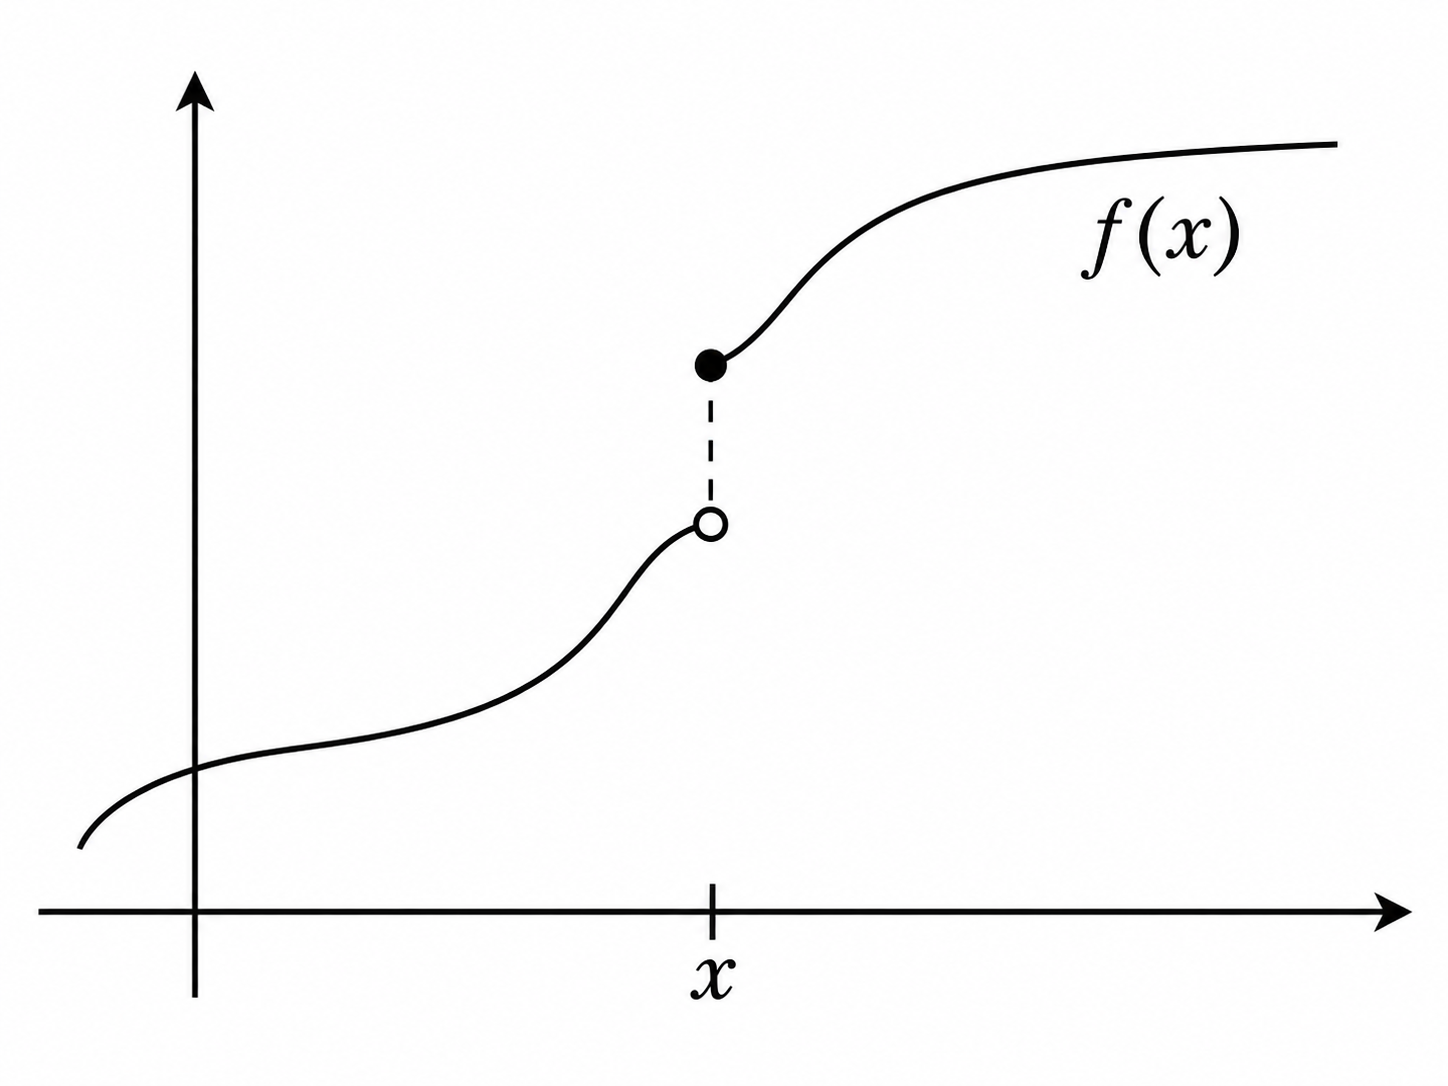
\includegraphics[width=0.3\textwidth]{Diagrams/Topology_WK_2_Q3.png}
    \caption{Right-continuous function with a jump discontinuity at \(x\).}
\end{figure}
\\
The black "blob" in the graph is the point $(x, f(x))$.
\newpage
\noindent
To prove continuity of such a function using the $(\mathbb{R},\mathcal{U})$ topology we just need to show that if we take any $B \in \mathcal{U}$,
then $f^{-1}(B) \in \mathcal{U}$.\\
\\
\textcolor{red}{I am at a loss as to the next step!}

\newpage
\noindent
\section*{Exercise 5}
 Let \(A\) be a subset of a topological space
\(X\). Show that:
\begin{enumerate}
\item[i)] \(A^\circ=A\) if and only if \(A\) is open in \(X\).
\item[ii)] \(\overline{A}=A\) if and only if \(A\) is closed in \(X\).
\item[iii)] \(X\setminus\overline{A}=(X\setminus A)^\circ\).
\end{enumerate}
\vspace{1cm}
\noindent
\underline{Answer:}\\
\\
(i) $A^\circ = A \iff A \text{ is open}$. \\
(a) $A^\circ = A \implies A \text{ is open}$.  By definition:
\begin{align*}
 A^\circ = \bigcup_{O \subset A} O \subset A \;\;\;\;\;\;\;\;\; \text{where O is open} \tag{5.1}
\end{align*}
From (5.1) we see that $A^\circ$ is defined as the union of a collection of open sets - and so must be open.  As $A^\circ = A$, then
$A$ must be open.\\
\\
(b) $A \text{ open } \implies A^\circ=A$.  Well this is straight forward!  $A$ will be one of the $O$ in the union of (5.1).\\
\\
(ii) $\bar{A} = A \iff A \text{ is closed}$. \\
(a) $\bar{A} = A \implies A \text{ is closed}$.  By definition:
\begin{align*}
 A \subset \bar{A} = \bigcap_{C \supset A} C  \;\;\;\;\;\;\;\;\; \text{where C is closed and contains A} \tag{5.2}
\end{align*}
From (5.2) $\bar{A}$ is the intersection of a collection of closed sets and so must itself by closed.  With $\bar{A} = A$, we must conclude that $A$
is closed.\\
\\
(b) $A \text{ closed } \implies \bar{A}=A$.  If $A$ is closed it will be one od the $C \supset A$ in the intersection and then $\bar{A} = A$.\\
\\
(iii) $[\bar{A}]^c = (A^c)^\circ$.\\
From the definitions we know that: $A^\circ \subset A \subset \bar{A}$.\\
\\
If we now take the complements: $(A^\circ)^c \supset A^c \supset [\bar{A}]^c \implies (A^c)^\circ \supset [\bar{A}]^c$ (*), since $[\bar{A}]^c$ must be open
and $(A^c)^\circ$ is the largest open set in $(A^c)$.\\
\\
Now assume that $x \in (A^c)^\circ$, that means there is an open set $U$ such that: $x \in U \subset (A^c)$, i.e. $U \cap A = \emptyset$ and hence $x \notin \bar{A}$.
That is to say $x \in [\bar{A}]^c$ and hence: $(A^c)^\circ \subset [\bar{A}]^c$ (**).\\
\\
The two way inclusions (*) and (**) prove the required equality.



\newpage
\noindent
\section*{Exercise 6}
Let \(X\) be an uncountable set; define the
cocountable topology on \(X\) as
\begin{align*}
\mathcal{U}_{\mathrm{cocountable}}
=\{U\subseteq X;\ X\setminus U\text{ is finite or countable}\}
\cup\{\varnothing\}.
\end{align*}

\begin{enumerate}
\item[i)] Prove that one may not find a countable base for topology
\(\mathcal{U}_{\mathrm{cocountable}}\) on \(X\).

\item[ii)] Show that if \(x_n\to x\) (in the cocountable topology),
then the sequence \(x_n\) stabilizes to \(x\) (i.e., there exists
\(N\in\mathbb{N}\) such that \(x_n=x\) for all \(n>N\)).

Recall the definition of sequentially convergence in topology:
\(x_n\to x\) in topology \((X,\mathcal{U})\), if for every neighborhood
\(U\) of \(x\) in \((X,\mathcal{U})\), there exists \(N\in\mathbb{N}\)
such that \(x_n\in U\) for all \(n>N\).

\item[iii)] Consider the identity function
\(I_{\mathbb{R}}:(\mathbb{R},\mathcal{U}_{\mathrm{cocountable}})
\to(\mathbb{R},\mathcal{U}_{\mathbb{R}})\), where
\(\mathcal{U}_{\mathbb{R}}\) denotes the Euclidean topology induced
by the metric \(d(x,y)=|x-y|\). Prove that \(I_{\mathbb{R}}\) is not
continuous; however, the image of every converging sequence converges
(i.e., \(I_{\mathbb{R}}\) is \emph{sequentially continuous}.)
\end{enumerate}
\vspace{1cm}
\underline{Answer:}\\
\\
Note: I use $\mathcal{U}$ for $\mathcal{U}_{cocountable}$.\\
\\
(i) Let
\begin{align*}
B \subset \mathcal{U}
= \{u \subset X \mid X-u \text{ is finite/countable}\}
\cup \{\emptyset\}
\end{align*}
be a base for $\mathcal{U}$.\\
Then it is clear that each $b \in B$
must be uncountable.
Now assume that $B$ itself is countable - i.e.
\begin{align*}
B=(b_i)_{i\in\mathbb{N}} \;\;\;\;\;\;\;\;\; \text{(and $\{\ \emptyset \} \notin B$ for simplicity)}
\end{align*}
From each $b_i$ select an element $c_i$.\\
Then $(c_i)_{i\in\mathbb{N}}$ is a sequence that contains at
least one element from each $b_i$.\\
Define
\begin{align*}
C=\{c_1,c_2,\ldots\}
\end{align*}
which is countable.\\
\\
As:
\begin{align*}
C=X \setminus (X \setminus C)
\end{align*}
It is clear that $X \setminus C$ is open and hence $(X-C) \in \mathcal{U}$.\\
But, from the definition of a base for $\mathcal{U}$, there is an index $I\subset\mathbb{N}$ s.t
\begin{align*}
X \setminus C=\bigcup_{i\in I} b_i
\end{align*}
This is a contradiction as $X \setminus C$ does not contain the $(c_i)_{i\in I}$.\\
\qed\\
\\
(ii) Let $x_n \to x$. Then for any $U \in \mathcal{U}, \;\;\; \exists N \in \mathbb{N}$ s.t.:,
\begin{align*}
 x_n \in U,\ \forall n>N \quad \& \quad x\in U
\end{align*}
Assume that $(x_n)$ never stabilizes to $x$. \\
Let:
\begin{align*}
D=\{x_n \mid x_n\neq x\}
\end{align*}
and $D$ is countably infinite.\\
Hence: $(X \setminus D)\in\mathcal{U}$, i.e. we have found an
open set in $\mathcal{U}$ s.t.
\begin{align*}
x\in(X \setminus D)\in\mathcal{U}
\end{align*}
but, by the definition of $D$:
\begin{align*}
\nexists N\in\mathbb{N}\text{ s.t.}
\end{align*}
\begin{align*}
x_n\in (X \setminus D) \qquad \forall n>N
\end{align*}
Contradiction. Hence $x_n$ must stabilize to $x$ at
some finite $n\in\mathbb{N}$.\\
\qed \\
\\
(iii) The identity function: $f: (\mathbb{R}, \mathcal{U}) \to (\mathbb{R}, \mathcal{U}_{\mathbb{R}})$, where $f(x)=x$, with the
two given topologies is not continuous.\\
\\
To demonstrate this we can take an open set in $\mathcal{U}_{\mathbb{R}}$ and show that its inverse
image is NOT an open set in $\mathcal{U}$.\\
\\
Take $(0,1) \in \mathcal{U}_{\mathbb{R}}$, clearly $f^{-1}((0,1)) = (0,1)$.
However, $\mathbb{R} \setminus (0,1)$ is not a countable set - and hence not open in $\mathcal{U}$.\\
\qed


\end{document}
